\documentclass[11pt,a4paper]{article}

\usepackage[UTF8]{ctex}
\usepackage{amsmath,amssymb,amsfonts}
\usepackage{graphicx}
\usepackage{booktabs}
\usepackage{multirow}
\usepackage{hyperref}
\usepackage{url}
\usepackage{algorithm}
\usepackage{algorithmic}
\usepackage{xcolor}
\usepackage{subcaption}
\usepackage[margin=2.5cm]{geometry}

\newcommand{\method}{React\_FM}

\title{\textbf{React\_FM: 面向 LLM 智能体在线适应的失败触发循环内记忆}}
\author{匿名作者}
\date{}

\begin{document}
\maketitle

\begin{abstract}
基于大语言模型（LLM）的 ReAct 框架智能体在反复遇到相同任务实例时，常常重复相同的错误，缺乏从过去失败中实时学习的机制。现有的经验记忆方法（如 Reflexion）仅在 episode 边界注入反思，无法在执行过程中进行中途修正。我们提出 \method{}——一种面向重复实例在线适应场景的失败触发循环内记忆系统：在执行过程中检测失败，通过混合 BM25-嵌入检索找到相关的过去失败-恢复经验，并将纠正性指导注入智能体的下一步推理中。在五个基准测试——ALFWorld、WebShop、ScienceWorld、HotPotQA 和 ToolBench——上进行评估，\method{} 在 ALFWorld 上取得最高成功率，并在不同失败模式的任务中保持竞争力。在 ScienceWorld Step~4 no-gate 正式协议（12 个核心任务类型上的 111 个 episodes）中，ExpeL 取得最高成功率（49.55\%，57.78 原始平均分）；online \method{} 达到 41.44\% 成功率和最高的原始平均分（64.25），优于 offline memory（39.64\%, 48.83）、ReAct baseline（37.84\%, 47.21）和 corrected Reflexion（36.94\%, 49.39），且无需预先完整收集一个 epoch 的经验。在短时域或策略主导的基准（WebShop、ToolBench）上，ExpeL 等 Episode 级方法仍具竞争力或更优，表明两类方法互补而非一方普遍占优。WebShop 上的跨环境迁移实验表明，共享记忆仅需单个 Epoch 即可达到每环境 Epoch 2 的性能。进一步在 HotPotQA 和 ToolBench 上的实验揭示，跨环境共享的有效性取决于任务同质性：同质任务正迁移，异质任务（如不同 API）则产生负迁移（$-$19.9\%），表明共享记忆应基于任务相似性选择性启用。
\end{abstract}

\section{引言}

大语言模型智能体在交互式环境中展现了出色的能力，从家居任务完成~\cite{shridhar2021alfworld}到网页导航~\cite{yao2022webshop}、科学实验~\cite{wang2022scienceworld}、多跳问答~\cite{yang2018hotpotqa}和 API 工具调用~\cite{qin2023toolllm}。ReAct 框架~\cite{yao2023react}通过交替进行推理和行动成为此类智能体的标准范式。然而，一个持续存在的局限性是：当智能体遇到失败——例如试图从一个关闭的容器中取出物品——它缺乏利用类似过去经验的机制，经常在不同 episode 中重复同样的错误。

近期的工作引入了经验记忆来解决这一局限。Reflexion~\cite{shinn2023reflexion}在失败的 episode 结束后生成自由文本反思，并在后续试次开始时注入。ExpeL~\cite{zhao2024expel}从轨迹池中提取跨任务的经验洞察。\textbf{这些方法有一个共同的设计选择：记忆在 episode 边界注入}——要么在新试次开始时，要么在任务切换时。虽然有效，但这种设计意味着智能体必须完成（或放弃）整个 episode 才能从经验记忆中获益，即使中途已经有失败信号可用。

我们将此识别为现有经验记忆系统在\textbf{检索时机（retrieval timing）}上的根本性局限。借鉴 Liu et al.~\cite{liu2025memory}提出的分类法——该分类法从形式、功能和动态三个维度对智能体记忆进行分类——我们观察到现有工作主要使用\emph{被动}检索时机：无论智能体当前状态如何，在固定时间点注入记忆。相反，我们提出\emph{主动的、失败触发的检索}：智能体监控自身的执行过程以发现失败信号，仅在需要时检索相关记忆。

我们提出 \method{}，一种面向 ReAct 智能体的失败触发循环内记忆系统。\method{} 通过三个机制运作：(1)~失败检测器，识别执行过程中的\emph{显式失败}（环境错误信号）和\emph{隐式失败}（执行成功但未取得进展的动作）；(2)~混合检索系统，使用 BM25 和句子嵌入与倒数排名融合（RRF）来找到相关的过去失败-恢复经验；(3)~后 episode 提取器，从轨迹中提炼失败-恢复对为结构化记忆条目。

我们在五个基准测试上评估 \method{}：ALFWorld（134 个环境）、WebShop（100 个会话）、ScienceWorld（Step~4 no-gate 正式协议：12 个核心任务类型上的 111 个 test episodes）、HotPotQA（500 个问题）和 ToolBench（765 个查询）。我们研究的是\emph{在线适应重复任务实例}的场景——智能体在不同 epoch 中遇到相同或相似的环境并积累经验。这一场景具有实际意义：家用机器人反复与同一厨房交互、客服智能体处理重复的查询类型、实验室助手执行相同的实验方案。\method{} 在 ALFWorld 上取得最高成功率；在 ScienceWorld 正式协议下，ExpeL 取得最高成功率（49.55\%, 57.78），而 online \method{} 达到 41.44\% 成功率和最高原始平均分 64.25，优于 ReAct baseline（37.84\%, 47.21）和 corrected Reflexion（36.94\%, 49.39）。在策略性或外部失败为主的基准（HotPotQA、ToolBench）上，ExpeL 等 Episode 级方法更为有效，揭示了互补而非普遍优越的适用场景。

\textbf{我们的贡献：}
\begin{itemize}
    \item 提出面向 ReAct 智能体的失败触发循环内记忆检索，实现基于过去经验的中途修正。在 ScienceWorld Step~4 正式协议下，online \method{} 达到 41.44\% 成功率和 64.25 原始平均分，优于 offline memory（39.64\%, 48.83）、ReAct baseline（37.84\%, 47.21）和 corrected Reflexion（36.94\%, 49.39）；ExpeL 在完成 Epoch 1 轨迹收集后于 Epoch 2 达到最高成功率（49.55\%, 57.78）。
    \item 提出结构化的失败-恢复记忆格式——存储（失败动作、观察、纠正动作）三元组。消融研究显示该格式比 Reflexion 风格反思高 +3.7\%（$p{=}0.056$，边缘显著），比成功轨迹的优势为方向性但不显著（$p{=}0.428$）。我们将格式和检索视为有前景的设计选择而非已经充分验证的独立贡献。
    \item 作为实现选择，我们结合 BM25 和句子嵌入检索并通过 RRF 融合，配合每环境记忆隔离。在 ALFWorld 上，混合方法匹配仅 BM25 的表现；跨基准的检索方法评估留作未来工作。
    \item 在五个基准上进行评估，并与强基线比较。\method{} 在 ALFWorld 上取得最高成功率，并在 ScienceWorld 正式 no-gate 协议中取得最高原始平均分；ExpeL 在 ScienceWorld、WebShop、HotPotQA 和 ToolBench 上取得最高成功率。跨三个基准的跨环境记忆迁移实验揭示任务同质性是迁移效果的关键预测因子：同质任务（WebShop）仅用单个 Epoch 即达 Epoch 2 性能，而异质任务（ToolBench）产生负迁移，表明共享记忆应选择性启用。
\end{itemize}

\section{相关工作}

\paragraph{交互式环境中的 LLM 智能体。} ReAct 框架~\cite{yao2023react}建立了将思维链推理与环境动作交替进行的范式，在知识密集型和决策任务上展现了强大性能。ALFWorld~\cite{shridhar2021alfworld}提供文本化家居环境，WebShop~\cite{yao2022webshop}测试产品搜索和购买，ScienceWorld~\cite{wang2022scienceworld}挑战多步科学实验。这些基准共享一个模式：智能体执行动作序列，早期错误级联导致失败，使错误恢复成为关键能力。

\paragraph{LLM 智能体的经验记忆。} 遵循 Liu et al.~\cite{liu2025memory}的分类法，智能体的经验记忆可分为：基于案例的（存储原始轨迹）、基于策略的（存储洞察和规则）和基于技能的（存储可复用的动作序列）。Reflexion~\cite{shinn2023reflexion}在失败 episode 后生成自由文本自我反思，注入后续试次——一种 episode 级注入的策略型记忆。ExpeL~\cite{zhao2024expel}提取跨任务经验洞察。R2D2~\cite{zheng2024r2d2}结合推理与检索。REMEMBERER~\cite{majumder2023rememberer}通过自然语言查询检索长期经验记忆。\textbf{所有这些方法共享一个设计：记忆在 episode 边界注入。没有任何方法支持由实时失败检测触发的中途检索。}

\paragraph{记忆检索时机。} Liu et al.~\cite{liu2025memory}区分被动检索（固定间隔或每步触发）和主动检索（特定条件触发）。大多数现有系统使用被动时机。基于失败信号的主动检索仍未被充分探索。我们的工作填补了这一空白，提出失败触发检索：智能体监控执行过程中的失败模式，仅在检测到失败时检索相关记忆，避免不必要的检索开销同时实现及时修正。

\section{方法}

\method{} 通过三个组件增强标准 ReAct 智能体：失败检测器、带混合检索的记忆存储和后 episode 记忆提取器。图~\ref{fig:architecture}展示了整体流程。

\begin{figure}[t]
    \centering
    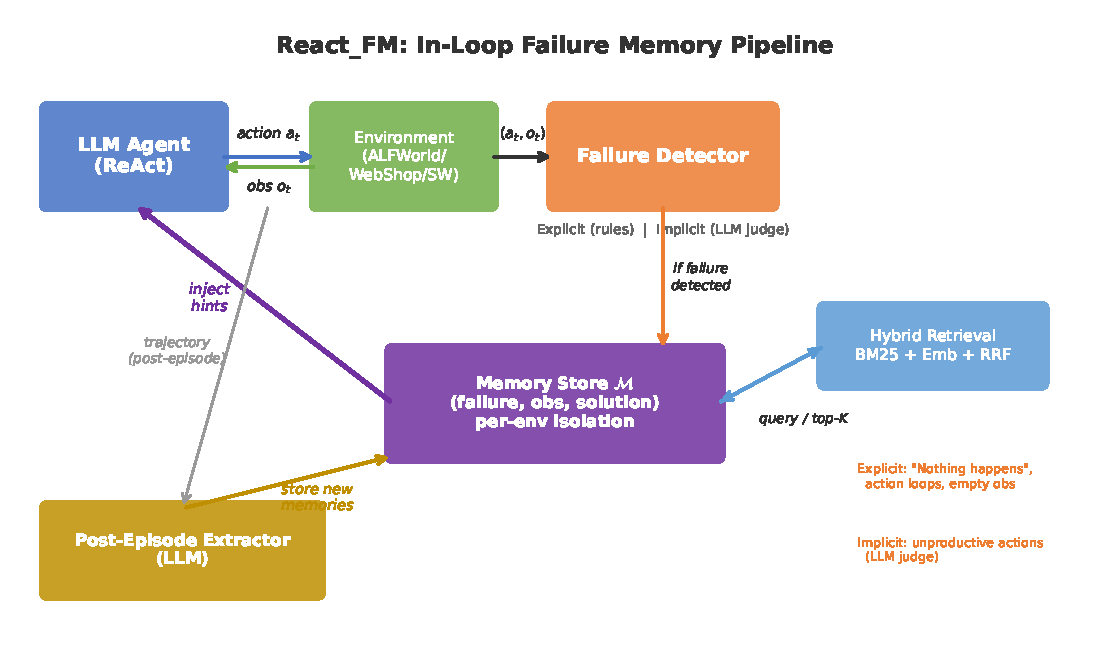
\includegraphics[width=\linewidth]{figures/architecture.pdf}
    \caption{\method{} 概述。每一步中，失败检测器监控动作-观察对以发现显式失败（环境错误）和隐式失败（无成效动作）。检测到失败时，通过混合 BM25-嵌入检索找到相关的过去经验并注入智能体提示。每个 episode 结束后，单独的 LLM 从轨迹中提取失败-恢复对并存储到每环境记忆中。}
    \label{fig:architecture}
\end{figure}

\subsection{问题形式化}

我们考虑一个智能体在离散时间步上与部分可观察环境交互。在步骤 $t$，智能体观察 $o_t$，基于历史 $h_t = (o_0, a_0, \ldots, o_{t-1}, a_{t-1}, o_t)$ 选择动作 $a_t$，并接收观察 $o_{t+1}$。智能体维护记忆存储 $\mathcal{M}$，包含来自过去 episode 的失败-恢复条目。关键问题是\emph{何时}以及\emph{如何}在执行过程中利用 $\mathcal{M}$。

\subsection{失败检测}

当智能体与环境交互时，失败以两种根本不同的形式出现：

\paragraph{显式失败。} 环境直接返回错误信号，表明动作无效或没有效果。例如错误消息（ALFWorld 中的 ``Nothing happens''，ScienceWorld 中的 ``No known action''）、空观察、以及同一动作连续重复 $k$ 次（$k{=}3$）无状态变化的动作循环。我们通过零成本的模式匹配规则来检测。

\paragraph{隐式失败。} 动作正常执行且没有报错，但结果并未解决智能体的预期目标。例如导航到已经访问过的位置，或拿起与任务无关的物品——环境正常响应，但没有取得有意义的进展。检测隐式失败需要理解动作背后的\emph{意图}，我们通过一个轻量级 LLM 判断器来评估每个动作-观察对是否``有成效''。

两种检测机制按顺序应用：显式失败规则首先运行（零成本），LLM 判断器仅在未检测到显式失败时调用（摊销成本）。

\subsection{记忆存储与混合检索}

\method{} 的一个关键设计选择是\textbf{存什么}。现有系统主要存储从成功中获得的知识：Reflexion 存储总结问题的自由文本反思，ExpeL 通过对比轨迹提取抽象洞察规则，REMEMBERER 存储成功轨迹片段。这些表示是\emph{抽象的}——智能体需要推理如何将一般性洞察应用到具体情境。

相反，\method{} 存储结构化\textbf{失败-恢复对}：
\begin{equation}
    m = (\textit{failure\_action}, \textit{failure\_observation}, \textit{solution\_action}, \textit{task\_type}, \textit{env\_idx})
\end{equation}

这种设计有三个优势。第一，\textbf{检索精度高}：失败场景稀疏且有辨别力，提供天然的检索锚点。第二，\textbf{可操作性强}：\texttt{solution\_action} 字段包含具体纠正步骤（如 ``open fridge 1 $\to$ take apple 1 from fridge 1''），智能体可直接参考。第三，\textbf{与检索时机对齐}：由于检索由失败触发，以失败为索引的记忆在存储键和检索查询之间建立天然对应。近期 ERL~\cite{chen2026erl}的工作也证实了这一设计，发现失败派生的启发式规则显著优于成功派生的。

每个环境维护独立的记忆存储。

\paragraph{混合检索。} 给定检测到的失败（动作 $a$ 和观察 $o$），构造查询 $q = a \| o$，使用两种互补方法检索：
\begin{itemize}
    \item \textbf{BM25}（词法）：通过词频重叠排序，有效匹配特定物品名称和动作模式。
    \item \textbf{句子嵌入}（语义）：使用 all-MiniLM-L6-v2 计算余弦相似度，捕捉语义相似性。
\end{itemize}

两个排名通过倒数排名融合（RRF）~\cite{cormack2009reciprocal}组合：
\begin{equation}
    \text{RRF}(m) = \sum_{r \in \{r_{\text{BM25}}, r_{\text{emb}}\}} \frac{1}{k + r(m)}
\end{equation}
其中 $r(m)$ 是条目 $m$ 在排名 $r$ 中的排名，$k{=}60$。返回 top-3 条目。

\subsection{循环内记忆注入}

当失败检测器触发且检索返回相关条目时，检索到的记忆被格式化并附加到智能体的提示中。此注入是\emph{瞬时的}：仅出现在失败后的下一个提示中，后续步骤移除，防止提示膨胀。

\subsection{后 Episode 记忆提取}

每个 episode 结束后，单独的 LLM（提取器）分析轨迹以识别失败-恢复模式：动作失败、智能体采取纠正步骤、最终目标达成的序列。存储为结构化 $(failure\_action, failure\_observation, solution\_action)$ 三元组。

\subsection{整体算法}

算法~\ref{alg:reactfm}总结了单个 episode 的 \method{} 执行流程。

\begin{algorithm}[t]
\caption{\method{} Episode 执行}
\label{alg:reactfm}
\begin{algorithmic}[1]
\REQUIRE 环境 $\mathcal{E}$，记忆存储 $\mathcal{M}$，最大步数 $T$
\STATE $o_0, \textit{task\_type} \leftarrow \mathcal{E}.\text{reset}()$
\STATE $h \leftarrow [o_0]$; $\textit{hints} \leftarrow \emptyset$
\FOR{$t = 0$ to $T-1$}
    \STATE $a_t \leftarrow \text{LLM}(h, \textit{hints})$ \COMMENT{生成动作}
    \STATE $\textit{hints} \leftarrow \emptyset$ \COMMENT{清除瞬时注入}
    \STATE $o_{t+1} \leftarrow \mathcal{E}.\text{step}(a_t)$
    \IF{$\text{ExplicitFail}(o_{t+1})$ \OR $\text{ImplicitFail}(a_t, o_{t+1})$}
        \STATE $\textit{hints} \leftarrow \mathcal{M}.\text{retrieve}(a_t, o_{t+1})$ \COMMENT{RRF 检索}
    \ENDIF
    \STATE $h \leftarrow h \cup \{(a_t, o_{t+1})\}$
    \IF{$\mathcal{E}.\text{done}()$}
        \STATE \textbf{break}
    \ENDIF
\ENDFOR
\STATE $\text{pairs} \leftarrow \text{Extract}(h)$ \COMMENT{LLM 提取器}
\STATE $\mathcal{M}.\text{add}(\text{pairs})$ \COMMENT{存储供未来 epoch 使用}
\end{algorithmic}
\end{algorithm}

\section{实验}

\subsection{实验设置}

\paragraph{基准测试。} 我们在五个不同的交互式环境上进行评估：
\begin{itemize}
    \item \textbf{ALFWorld}~\cite{shridhar2021alfworld}：文本化家居任务（拿放、清洁、加热、冷却、检查、拿两个），使用 \texttt{eval\_out\_of\_distribution} 划分，134 个环境，6 种任务类型。
    \item \textbf{WebShop}~\cite{yao2022webshop}：电子商务产品搜索与购买。100 个会话，1000 种产品。成功度量：奖励（0--1 规模），成功率定义为奖励 $\geq 0.5$。
    \item \textbf{ScienceWorld}~\cite{wang2022scienceworld}：文本化科学实验模拟，30 种任务类型。本文使用 Step~4 no-gate 正式协议：12 个核心任务类型上的 111 个 test episodes，每个任务最多 10 个 test variations，报告成功率和 ScienceWorld 原始平均分。
    \item \textbf{HotPotQA}~\cite{yang2018hotpotqa}：多跳问答任务。智能体使用 Search、Lookup 和 Finish 动作在多篇 Wikipedia 文章中查找并综合信息。500 个验证集样本，报告精确匹配（EM）和 F1 分数。
    \item \textbf{ToolBench}~\cite{qin2023toolllm}：基于 StableToolBench~\cite{guo2024stabletoolbench} 的 API 工具调用基准，765 个可解查询，跨 6 个子集（G1--G3）。智能体调用真实 API 函数回答用户查询。报告通过率（智能体通过 Finish 动作提交非空答案）。
\end{itemize}

\paragraph{对比系统。}
\begin{itemize}
    \item \textbf{ReAct Baseline}：标准 ReAct + few-shot 提示，无记忆。
    \item \textbf{Reflexion}~\cite{shinn2023reflexion}：Episode 级自我反思，注入试次开始。两轮试次：第一轮收集失败，第二轮利用反思。ScienceWorld Step~4 中报告修正后的最终指标：若 pass~0 已成功，则沿用 pass~0；否则使用真实 pass~1。
    \item \textbf{ExpeL}~\cite{zhao2024expel}：通过对比成功和失败轨迹提取跨任务洞察规则。Epoch 1 后提取抽象规则，Epoch 2 在 episode 开始时注入。使用相同 LLM 骨干复现以确保公平比较。
    \item \textbf{Offline memory（仅 ScienceWorld）}：Step~4 runbook 中的两阶段变体。先在 ScienceWorld train split 上收集 memory 且不做检索，再在 test split 上启用循环内检索评测。
    \item \textbf{\method{}}：我们的失败触发循环内记忆系统。多 epoch 基准报告 Epoch 1（首轮，构建记忆）和 Epoch 2（含 Epoch 1 累积记忆）；ScienceWorld Step~4 中报告从空 memory 开始的在线单次 test stream。
\end{itemize}

\paragraph{实现细节。} ALFWorld 和 WebShop 使用 Qwen3.5-9B 作为智能体 LLM 和失败判断器。DeepSeek-V3.2 用作记忆提取器（ALFWorld/WebShop）及 ScienceWorld、HotPotQA 和 ToolBench 的智能体 LLM（复杂推理需要更强模型）。所有 LLM 通过 SiliconFlow API 访问。句子嵌入使用本地 all-MiniLM-L6-v2。记忆检索使用 BM25 + 嵌入 + RRF（$k{=}60$），返回 top-3。每 episode 最大步数：50（ALFWorld）、15（WebShop）、8（HotPotQA）、12（ToolBench）。ScienceWorld Step~4 使用专门的 100-step limit；该正式协议关闭隐式 LLM 判断器，依赖显式规则检测，因此 ScienceWorld 主结果不计判断器 token。

\subsection{主要结果}

\begin{table}[t]
\centering
\caption{共享同一 multi-epoch 协议的四个基准测试主要结果。展示 95\% Bootstrap 置信区间（10K 重采样）。Tok 为每环境总 token 消耗（千），包含所有轮次的智能体、判断器和提取器开销。\textbf{粗体}为最优结果。ScienceWorld 使用单独的 Step~4 no-gate 正式协议，见表~\ref{tab:sw_step4}。}
\label{tab:main_results}
\scriptsize
\setlength{\tabcolsep}{1.6pt}
\begin{tabular}{l cc ccc ccc cc}
\toprule
\multirow{2}{*}{系统} & \multicolumn{2}{c}{ALFWorld} & \multicolumn{3}{c}{WebShop} & \multicolumn{3}{c}{HotPotQA} & \multicolumn{2}{c}{ToolBench} \\
\cmidrule(lr){2-3} \cmidrule(lr){4-6} \cmidrule(lr){7-9} \cmidrule(lr){10-11}
 & 成功 & Tok & 成功 & 奖励 & Tok & EM & F1 & Tok & 通过 & Tok \\
\midrule
Baseline & 91.0\tiny{[86,96]} & 52.9 & 38.0\tiny{[29,47]} & .38 & 38.3 & .40 & .50 & 5.5 & 62.8 & 6.3 \\
Reflexion & 94.0\tiny{[90,98]} & 53.8 & 45.0\tiny{[35,55]} & .41 & 41.8 & .44 & .53 & 6.1 & 81.4 & 5.6 \\
ExpeL & 94.8\tiny{[91,99]} & 50.8 & \textbf{49.0}\tiny{[39,59]} & \textbf{.44} & 38.8 & \textbf{.44} & \textbf{.54} & 6.1 & \textbf{90.6} & 4.9 \\
\midrule
\method{} E1 & 91.8 & 56.4 & 40.0 & .39 & 46.0 & .40 & .49 & 7.2 & 62.1 & 7.7 \\
\method{} E2 & \textbf{95.5}\tiny{[92,99]} & 53.5 & 44.0\tiny{[34,54]} & .42 & 45.2 & .43 & .52 & 7.1 & 75.3 & 7.1 \\
\bottomrule
\end{tabular}
\vspace{0.3em}

{\footnotesize Tok = 每任务平均有效 token 消耗（K）：对每个任务，计算产出其最终结果的轮次的 token（E1 成功则计 E1，需重跑则计 E2），再对所有 $N$ 个任务取平均。Reflexion/ExpeL 报告最终轮次（Trial 1 / Epoch 2）。}
\end{table}

表~\ref{tab:main_results}展示了共享同一 multi-epoch 协议的四个基准结果。\method{} 在 ALFWorld 上取得最高成功率。在策略性或外部失败为主的基准上，Episode 级方法仍然更强。

\paragraph{ScienceWorld agent-memory 结果定位。}
现有 ScienceWorld memory / experience-based agent 结果很难直接比较，因为不同工作使用的 task subset、variant 采样方式、模型 backbone 和 adaptation 协议都不一致。有些方法评测全部 30 个 task types，有些使用 18-task 子集或少数任务类别；一些较强结果还依赖 multi-trial test-time self-improvement、skill library、golden trajectories、训练后的 planner 或 long-context trajectory conditioning。因此，我们将已有 ScienceWorld 结果作为背景参考，而不是作为 leaderboard 式横向排名。我们的 ScienceWorld 实验采用受控的 within-protocol comparison：所有方法都在相同的 12 个核心 task types、111 个 test episodes、相同 split、variation cap、step limit 和 backbone 设置下评测。

\begin{table}[t]
\centering
\caption{ScienceWorld Step~4 no-gate 正式对比实验，包含 12 个核心 task types 上的 111 个 test episodes。Avg Score 使用 ScienceWorld 原始分数尺度。Reflexion P1 Adj 是修正后的最终指标；ExpeL 报告从 Epoch~1 提取 insights 后的 Epoch~2 结果。}
\label{tab:sw_step4}
\small
\setlength{\tabcolsep}{4pt}
\begin{tabular}{lccc}
\toprule
方法 & 成功率 & 平均分 & Tok/ep (K) \\
\midrule
ReAct baseline & 37.84\% & 47.21 & 185.5 \\
Reflexion P0 & 25.23\% & 40.57 & 111.7 \\
Reflexion P1 Adj & 36.94\% & 49.39 & 212.6 \\
Offline memory & 39.64\% & 48.83 & 180.4 \\
\method{} online & 41.44\% & \textbf{64.25} & 197.2 \\
\textbf{ExpeL} & \textbf{49.55\%} & 57.78 & 190.9 \\
\bottomrule
\end{tabular}
\end{table}

\paragraph{ALFWorld。} \method{} (E2) 达到 95.5\% 成功率，为所有系统中最高。配对 Bootstrap 检验（10K 重采样，双侧）显示：vs 基线 $p{=}0.069$，vs ExpeL $p{=}0.859$，vs Reflexion $p{=}0.601$。在 $n{=}134$ 下，\method{} 相对 ExpeL 和 Reflexion 的优势不具统计显著性，但 \method{} 通过循环内修正实现改进，无需重启 episode 或跨轨迹对比。

\paragraph{WebShop。} \method{} 从 38.0\%（基线）提升到 44.0\%（+6.0\%，$p{=}0.051$），平均奖励从 0.381 到 0.416。ExpeL 在该基准上取得最高成功率（49.0\%），其次是 Reflexion（45.0\%）。对于短时域、任务结构统一的购物任务，Episode 级抽象洞察（ExpeL）或反思（Reflexion）可能比循环内失败-恢复对更有效。

\paragraph{ScienceWorld。} 表~\ref{tab:sw_step4}展示了 ScienceWorld Step~4 no-gate 正式对比实验结果。在这一受控协议下，ExpeL 在 Epoch 2 达到最高成功率（49.55\%，原始平均分 57.78），而 online \method{} 达到 41.44\% 成功率和最高原始平均分 64.25。相比 ReAct baseline，\method{} 的成功率提升 +3.60 个百分点，平均分提升 +17.04；相比 corrected Reflexion 和 Offline memory，\method{} 也取得更高平均分，同时不需要 episode restart 或预先完成一个完整收集 epoch。ExpeL 的结果说明完整轨迹后的抽象 insight 对 ScienceWorld 成功率很有效；\method{} 的结果则说明在线循环内记忆能在单次 test stream 中改善局部进展。

\paragraph{HotPotQA。} \method{} 将 EM 从 0.396（基线）提升到 0.430（+3.4\%），F1 从 0.502 提升到 0.515。E1$\to$E2 的提升（EM 0.395$\to$0.430）来自 skip-on-success 机制：E1 中正确回答的问题在 E2 中直接沿用，而失败的问题用每环境记忆重新尝试。Reflexion（EM=0.441）和 ExpeL（EM=0.440，F1=0.535）略优于 \method{}，这与离线反思方法在问答任务中受益于完整 episode 回顾分析的模式一致。跨环境记忆共享（\S\ref{sec:cross_env}）通过在不同问题间迁移程序性模式，在单个 Epoch 内提供了中度改善（EM 0.395$\to$0.408）。

\paragraph{ToolBench。} \method{} 从 62.1\%（E1）提升到 75.3\%（E2），比基线（62.8\%）高 +12.5\%。然而 Reflexion（81.4\%）和 ExpeL（90.6\%）达到更高的通过率。分析发现 ToolBench 的失败主要由 API 缓存未命中导致（StableToolBench 框架返回预缓存的 API 响应，新参数组合返回``无缓存响应''）——这是动作级记忆无法解决的外部限制。ExpeL 学到了``使用已有信息而非重试失败 API 调用''等抽象策略，对此失败模式更有效。尽管排名第三，\method{} 相对基线的大幅提升表明循环内记忆在主要失败模式为外部因素时仍能提供有意义的收益。

\paragraph{分离检测与检索的贡献。} 仅检测控制实验（\texttt{inject\_mode=none}）中，失败检测器激活但不注入记忆。在 ALFWorld 上，仅检测（93.3\%）优于基线（91.0\%）但低于完整系统（95.5\%），确认检索增加 +2.2\%。在 WebShop 上，仅检测（42.0\%）和完整系统（44.0\%）均优于基线，差距较小，说明检索提供了额外但较温和的收益。ScienceWorld 的最终正式协议不同于这些 multi-epoch 消融，因此我们不再将早期 pilot 消融作为主结论，而是在表~\ref{tab:sw_step4}中通过 online、offline memory、ReAct 和 Reflexion 的受控对比分析 memory 的作用。

\paragraph{ALFWorld 每任务分析。}
图~\ref{fig:per_task}展示了 ALFWorld 上的每任务分析。\method{} 在 \texttt{clean} 任务上取得了最大改进（+12.8\%），该类任务的常见失败模式——尝试从关闭的容器中取物——被记忆系统有效捕获。基线已达 100\% 的任务（\texttt{cool}、\texttt{put}）未出现退步。

\begin{figure}[t]
    \centering
    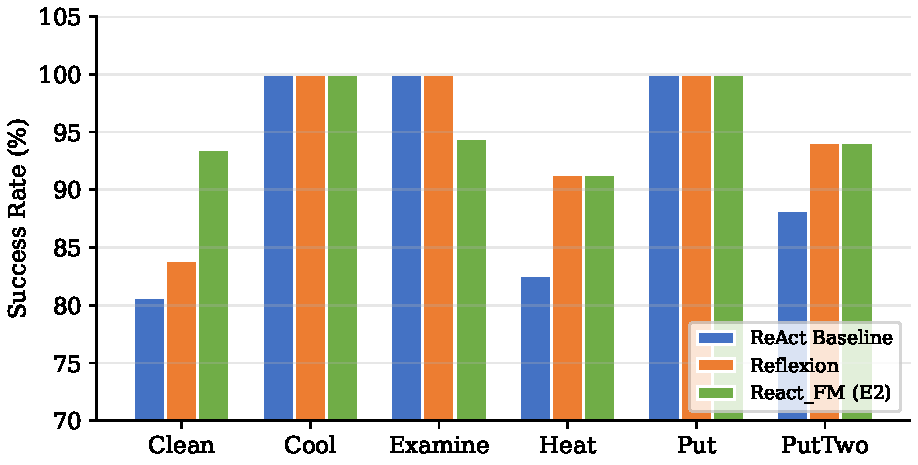
\includegraphics[width=\linewidth]{figures/alfworld_per_task.pdf}
    \caption{ALFWorld 每任务成功率。\method{} 在 \texttt{clean} 上提升最大（+12.8\%），除 \texttt{examine}（94.4\% vs 100\%）外，在所有任务类型上匹配或超越 Reflexion。}
    \label{fig:per_task}
\end{figure}

\paragraph{ScienceWorld 每任务分析。}
表~\ref{tab:sw_per_task}展示了 ScienceWorld Step~4 正式协议下的每任务分析。Online \method{} 并不支配所有任务类型。它相对 ReAct baseline 在 \texttt{melt}（+33.4 个百分点）、\texttt{grow-plant}（+30.0）、\texttt{power-component}（+40.0）和 \texttt{use-thermometer}（+10.0）上有明确改进；但 baseline 在 \texttt{inclined-plane-friction-unnamed-surfaces} 上仍然更强。ExpeL 在多个任务类型上成功率最高，尤其是 \texttt{melt}、\texttt{lifespan-longest-lived-then-shortest-lived}、\texttt{test-conductivity} 和 \texttt{use-thermometer}；但 \texttt{mendelian-genetics-unknown-plant} 仍是所有方法都未能解决的持续困难任务。这种 task-level heterogeneity 与 runbook 结论一致：memory 在 ScienceWorld 上有帮助，但收益强烈依赖任务类型，无条件干预并不是最优策略。

\begin{table}[t]
\centering
\caption{ScienceWorld Step~4 正式协议下的每任务成功率。}
\label{tab:sw_per_task}
\small
\setlength{\tabcolsep}{3pt}
\begin{tabular}{p{3.7cm}ccccc}
\toprule
任务 & Online & Offline & ReAct & Reflexion Adj & ExpeL \\
\midrule
boil & 33.3 & 33.3 & 44.4 & 11.1 & 44.4 \\
chemistry-mix & 37.5 & 37.5 & 25.0 & 25.0 & 37.5 \\
grow-plant & 30.0 & 30.0 & 0.0 & 30.0 & 50.0 \\
inclined-plane-friction-unnamed-surfaces & 40.0 & 50.0 & 60.0 & 50.0 & 30.0 \\
lifespan-longest-lived-then-shortest-lived & 50.0 & 60.0 & 50.0 & 40.0 & 70.0 \\
melt & 66.7 & 44.4 & 33.3 & 22.2 & 88.9 \\
mendelian-genetics-known-plant & 90.0 & 70.0 & 80.0 & 80.0 & 70.0 \\
mendelian-genetics-unknown-plant & 0.0 & 0.0 & 0.0 & 0.0 & 0.0 \\
power-component & 60.0 & 0.0 & 20.0 & 40.0 & 20.0 \\
test-conductivity & 10.0 & 10.0 & 20.0 & 30.0 & 40.0 \\
test-conductivity-of-unknown-substances & 0.0 & 20.0 & 30.0 & 20.0 & 30.0 \\
use-thermometer & 90.0 & 100.0 & 80.0 & 90.0 & 100.0 \\
\midrule
\textbf{Overall} & 41.44 & 39.64 & 37.84 & 36.94 & \textbf{49.55} \\
\bottomrule
\end{tabular}
\end{table}

\paragraph{WebShop 分析。}
WebShop 上的主要失败模式是：(1) 搜索查询过于具体导致返回结果少，(2) 选择产品时未检查所有要求的属性（颜色、尺寸、材料）。\method{} 通过存储失败-恢复对来应对这些问题。从 E1 到 E2 的渐进改进（+4\% 成功率，+0.031 平均奖励）表明这些模式在具有相似产品类别的购物会话间可以迁移。

\subsection{学习曲线}

\begin{figure}[t]
    \centering
    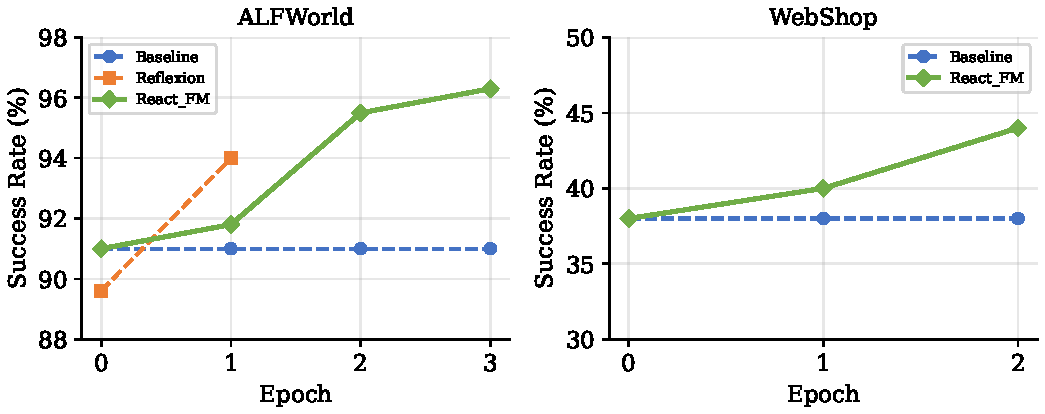
\includegraphics[width=\linewidth]{figures/learning_curve.pdf}
    \caption{ALFWorld 和 WebShop 上跨 epoch 的成功率变化。\method{} 随记忆积累持续改进，而基线保持不变。ALFWorld（左）上，\method{} 在 Epoch 2 超越 Reflexion。}
    \label{fig:learning_curve}
\end{figure}

图~\ref{fig:learning_curve}展示了 ALFWorld 和 WebShop 上跨 epoch 的学习曲线。模式一致：\method{} 随 epoch 持续改进，而基线保持不变。ALFWorld 上从 91.8\%（E1）到 95.5\%（E2）到 96.3\%（E3）。WebShop 从 E1 的 40.0\% 提升到 E2 的 44.0\%。在 HotPotQA 上，EM 从 0.395（E1）提升到 0.430（E2）；ToolBench 上通过率从 62.1\%（E1）提升到 75.3\%（E2），均通过 skip-on-success 机制实现。ScienceWorld 未放入该学习曲线，因为其最终结果采用专门的 Step~4 one-pass no-gate 协议，而不是早期 pilot multi-epoch 设置。跨环境记忆共享（\S\ref{sec:cross_env}）可在同质任务基准上进一步加速收敛。

\subsection{记忆分析}

\begin{table}[t]
\centering
\caption{ALFWorld Epoch 2 后的 \method{} 记忆统计。}
\label{tab:memory_stats}
\begin{tabular}{lcccccc}
\toprule
 & Clean & Cool & Examine & Heat & PutTwo & Put \\
\midrule
条目数 & 16 & 9 & 53 & 15 & 11 & 6 \\
\bottomrule
\end{tabular}
\vspace{0.5em}

\begin{tabular}{lccc}
\toprule
总条目数 & 有记忆的环境 & 检索次数 & 命中次数 \\
\midrule
110 & 43/134 & 212 & 44 (20.8\%) \\
\bottomrule
\end{tabular}
\end{table}

表~\ref{tab:memory_stats}报告了 ALFWorld 上的记忆统计。系统积累了 110 个失败-恢复条目，覆盖 43 个环境（32\% 的环境经历了至少一次检测到的失败）。\texttt{Examine} 任务产生了最多条目（53），与其复杂的多步骤性质一致。20.8\% 的检索命中率（44/212）表明选择性检索——记忆仅在存在相关匹配时才注入。

\paragraph{Token 效率。} WebShop 上，\method{} E2 使用 3.89M token，基线为 3.83M（+1.6\%），以最小开销换取 +6\% 成功率。在 ScienceWorld Step~4 正式协议上，online \method{} 每 episode 使用 197.2K token，baseline 为 185.5K（+6.3\%），同时成功率提升 +3.60 个百分点、平均分提升 +17.04。Offline memory 更省 token（180.4K/episode），而 corrected Reflexion 的真实运行成本下界为 212.6K/episode，因为 pass0 和 pass1 都实际执行。判断 LLM 增加 82K token（ALFWorld 智能体 token 的 4.7\%），提取器增加 24K（1.4\%），确认了轻量级特性。

\paragraph{失败检测分析。} 表~\ref{tab:detection_stats}总结了最终协议中启用隐式判断器的基准上的失败检测情况。在 ALFWorld 上，所有 56 次检测到的失败均为\emph{显式失败}（``Nothing happens''），通过零成本模式匹配检测，无 LLM 判断器调用——检测机制完全确定性。在 WebShop 上，49\% 的 episode 触发至少一次失败检测，隐式判断器开销为 94K token。ScienceWorld Step~4 正式协议关闭隐式 LLM 判断器，改用显式规则检测，因此主文不再报告 ScienceWorld 判断器 token 统计。

\paragraph{判断器精度审计。} 为验证隐式失败判断器，我们人工审计了 WebShop Epoch 2 中判断器触发的检测样本。我们检查了 30 个唯一（动作，观察）对：全部 30 个为真阳性——搜索查询返回指令页面而未导航到产品结果，被正确标记为无效（精度：100\%）。由于 ScienceWorld 最终 Step~4 协议不再使用隐式 LLM 判断器，我们不在主文报告对应的 ScienceWorld 判断器审计。

\paragraph{召回率局限。} 我们的审计衡量的是精度（检测到的失败中真实失败的比例），而非召回率（真实失败中被检测到的比例）。估算召回率需要标注一组 episode 中的所有动作-观察对，而非仅标注被判断器标记的——这是一项成本高得多的标注工作。我们注意到两个缓解因素：(1) 基于模式匹配的显式失败检测是确定性的，对其覆盖的失败类型（如 ALFWorld 中的 ``Nothing happens''）具有接近完美的召回率；(2) 所有基准上 E1$\to$E2 的一致改进间接表明检测器捕获了相当比例的失败，因为未被检测的失败无法贡献记忆积累。全面的召回率评估（含多位标注者）是未来工作的重要方向。

\begin{table}[h]
\centering
\caption{各基准上的失败检测统计（Epoch 2）。}
\label{tab:detection_stats}
\small
\begin{tabular}{lccccc}
\toprule
基准 & 有失败的 Episode & 总检测数 & 判断器 Token & 仅显式？ \\
\midrule
ALFWorld & 9/134 (6.7\%) & 56 & 0 & 是 \\
WebShop & 49/100 (49.0\%) & 567 & 94K & 否 \\
\bottomrule
\end{tabular}
\end{table}

\subsection{消融实验}
\label{sec:ablation}

我们设计消融实验来隔离 \method{} 的两个关键设计选择：(1) \emph{何时}注入记忆（检索时机），(2) \emph{存什么}（记忆格式）。时机、检测、格式和检索消融主要在 ALFWorld 和 WebShop 上评估。ScienceWorld 使用专门的 Step~4 正式协议进行分析，因为最终协议与早期 pilot multi-epoch 消融不同。

\paragraph{消融 1：检索时机。}
固定记忆格式（失败-恢复对），对比注入模式。表~\ref{tab:ablation_timing}展示 ALFWorld 和 WebShop 上的结果。

\begin{table}[h]
\centering
\caption{检索时机消融（Epoch 2）。所有变体使用相同的失败-恢复记忆格式。}
\label{tab:ablation_timing}
\small
\begin{tabular}{lccc}
\toprule
\multirow{2}{*}{注入模式} & \multicolumn{2}{c}{ALFWorld} & WebShop \\
\cmidrule(lr){2-3} \cmidrule(lr){4-4}
 & E1 & E2 & E2 \\
\midrule
无记忆（基线） & 91.0\% & --- & 38.0\% \\
Episode 级注入 & 90.2\% & 94.8\% & 45.0\% \\
\textbf{循环内注入（我们的）} & \textbf{91.8\%} & \textbf{95.5\%} & 44.0\% \\
\bottomrule
\end{tabular}
\end{table}

\paragraph{消融 2：记忆格式。}
固定注入模式（循环内），对比三种存储格式。表~\ref{tab:ablation_format}将该消融扩展到 ALFWorld 和 WebShop。

\begin{table}[h]
\centering
\caption{记忆格式消融（Epoch 2）。所有变体使用循环内注入时机。}
\label{tab:ablation_format}
\small
\begin{tabular}{lp{3cm}cccc}
\toprule
\multirow{2}{*}{记忆格式} & \multirow{2}{*}{存储内容} & \multicolumn{2}{c}{ALFWorld} & \multicolumn{2}{c}{WebShop} \\
\cmidrule(lr){3-4} \cmidrule(lr){5-6}
 & & E1 & E2 & E2 SR & E2 Rew \\
\midrule
成功轨迹 & 成功 episode 的关键步骤 & 91.8\% & 94.8\% & 48.0\% & .456 \\
Reflexion 反思 & 自由文本失败反思 & 89.6\% & 91.8\% & 46.5\% & .449 \\
\textbf{失败-恢复（我们的）} & (失败动作, 观察, 修复) & \textbf{91.8\%} & \textbf{95.5\%} & 44.0\% & .416 \\
\bottomrule
\end{tabular}
\end{table}

\paragraph{消融 3：检测 vs. 检索。}
为隔离失败检测与记忆检索的贡献，我们运行\emph{仅检测}控制实验（\texttt{inject\_mode=none}）：失败检测器激活但不注入检索到的记忆。在 ALFWorld 和 WebShop 上评估。

\begin{table}[h]
\centering
\caption{仅检测控制实验（Epoch 2 全集指标）。仅检测激活失败检测器但禁用记忆注入。}
\label{tab:detection_only}
\small
\begin{tabular}{lcc}
\toprule
系统 & ALFWorld & WebShop \\
\midrule
ReAct 基线 & 91.0\% & 38.0\% \\
仅检测 (E2) & 93.3\% & 42.0\% \\
\textbf{\method{} 完整 (E2)} & \textbf{95.5\%} & \textbf{44.0\%} \\
\bottomrule
\end{tabular}
\end{table}

在 ALFWorld 上，仅检测（93.3\%）优于基线（91.0\%）但低于完整系统（95.5\%），确认记忆检索在检测之外提供额外 +2.2\% 的增益。在 WebShop 上，仅检测（42.0\%）和完整系统（44.0\%）均优于基线，差距较小，说明检索提供了温和的额外收益。

\paragraph{消融 4：检索方法。}
固定其他组件（循环内注入，失败-恢复格式），对比三种检索方法。表~\ref{tab:retrieval_ablation}展示 ALFWorld 和 WebShop 上的结果。

\begin{table}[h]
\centering
\caption{检索方法消融（Epoch 2）。WebShop 结果来自部分运行（70/100 环境），因 API 可用性中断。}
\label{tab:retrieval_ablation}
\small
\begin{tabular}{lccc}
\toprule
\multirow{2}{*}{检索方法} & ALFWorld & \multicolumn{2}{c}{WebShop$^*$} \\
\cmidrule(lr){2-2} \cmidrule(lr){3-4}
 & E2 & E2 SR & E2 Rew \\
\midrule
仅 BM25 & 95.5\% & 41.4\% & .396 \\
仅嵌入 & 93.1\% & 40.0\% & .403 \\
\textbf{混合 RRF（我们的）} & \textbf{95.5\%} & \textbf{44.0\%} & \textbf{.416} \\
\bottomrule
\multicolumn{4}{l}{\footnotesize $^*$WebShop：70/100 环境完成。}
\end{tabular}
\end{table}

在 ALFWorld 上，混合 RRF（95.5\%）匹配仅 BM25（95.5\%）并优于仅嵌入（93.1\%）。BM25 的强表现反映了 ALFWorld 受限词汇下词法匹配的高效性。在 WebShop 上（部分结果，70/100 环境），混合 RRF（44.0\%）优于仅 BM25（41.4\%）和仅嵌入（40.0\%），表明混合方法在任务涉及多样化自然语言描述时提供更大收益。仅嵌入检索在两个基准上均表现较弱，可能因为失败描述共享相似语言模式时语义相似度区分度不足。

\textbf{检索时机}（表~\ref{tab:ablation_timing}）：跨基准结果揭示了循环内相对 Episode 级注入的优势是\emph{依赖于任务复杂度的}。在 ALFWorld 上，循环内注入（95.5\%）相比 Episode 级注入（94.8\%，$p{=}0.415$）有小幅提升——方向性正确但未达统计显著。在 WebShop 上，Episode 级（45.0\%）略优于循环内（44.0\%），表明对于短时域任务，前置指导可能已经足够。ScienceWorld Step~4 的 formal comparison 与 online in-loop memory 的有效性一致，但由于它同时改变了 memory 来源和评测协议，我们不将其解释为干净的 timing-only 消融。我们的结论是：\emph{失败触发的循环内检索在任务为长时域且失败模式多样且不可预测时最有价值}，而非声称对 Episode 级注入的普遍优势。

\textbf{记忆格式}（表~\ref{tab:ablation_format}）：在 ALFWorld 上，失败-恢复对（95.5\%）优于成功轨迹（94.8\%，$p{=}0.428$）和 Reflexion 风格反思（91.8\%，$p{=}0.056$）。有趣的是，在 WebShop 上模式逆转：成功轨迹（48.0\%）和 Reflexion 反思（46.5\%）均优于失败-恢复对（44.0\%）。这表明对于结构统一的短时域购物任务，高层指导（什么有效或什么应避免）可能比具体的失败-恢复序列更具可迁移性。ALFWorld 上失败-恢复对相对抽象反思的优势（+3.7\%，$p{=}0.056$）仍是最大的显著效应，与结构化可操作记忆对具有多样失败模式的长时域任务最有价值的假设一致。

\subsection{定性示例}

表~\ref{tab:examples}展示了 \method{} 在 ALFWorld 上提取的代表性失败-恢复对，说明三种常见失败模式：(1) 未打开容器就交互，(2) 在错误位置执行动作，(3) 操作顺序不正确。

\begin{table}[t]
\centering
\caption{\method{} 记忆存储中的代表性失败-恢复对（ALFWorld）。}
\label{tab:examples}
\small
\begin{tabular}{p{1.2cm}p{3.0cm}p{3.0cm}}
\toprule
类型 & 失败动作 $\to$ 观察 & 存储的解决方案 \\
\midrule
cool & \texttt{put tomato in microwave} $\to$ ``Nothing happens'' & \texttt{open microwave} $\to$ \texttt{put tomato in microwave} \\
\addlinespace
examine & \texttt{open drawer 2} $\to$ ``Nothing happens'' & \texttt{go to drawer 2} $\to$ \texttt{open drawer 2} \\
\addlinespace
clean & \texttt{clean towel with sink} $\to$ ``Nothing happens'' & \texttt{put towel in sink} $\to$ \texttt{clean towel with sink} \\
\bottomrule
\end{tabular}
\end{table}

\subsection{跨 Benchmark 讨论}

五个基准在不同条件下测试了 \method{}，混合的结果提出了一个关于失败触发循环内记忆的\emph{适用场景假说}。表~\ref{tab:regime}总结了关键特征。我们强调，这一适用场景分析是探索性的——基于五个存在干扰因素（不同骨干模型、不同任务结构）的基准的相关性分析——而非严格论证的运行规律。

\begin{table}[h]
\centering
\caption{探索性的适用场景分析。\method{} 在 ALFWorld 上最强，并在 ScienceWorld Step~4 正式 no-gate 协议上取得最高原始平均分；ExpeL 在 ScienceWorld 上取得最高成功率。$\Delta$ = \method{} 相对对应 baseline 指标的增益。}
\label{tab:regime}
\small
\setlength{\tabcolsep}{2pt}
\resizebox{\linewidth}{!}{%
\begin{tabular}{lcccl}
\toprule
基准 & 最大步数 & 主要失败 & $\Delta$ & 最优方法 \\
\midrule
ScienceWorld & 100 & 动作级、任务依赖 & +3.60 pp succ.; +17.04 score & ExpeL (succ.) / \method{} (score) \\
ALFWorld & 50 & 动作级 & +4.5 pp succ. & \method{} \\
ToolBench & 12 & 外部（API） & +12.5 pp pass & ExpeL \\
WebShop & 15 & 混合 / 短时域 & +6.0 pp succ. & ExpeL \\
HotPotQA & 8 & 策略级 & +3.4 pp EM & ExpeL \\
\bottomrule
\end{tabular}
}
\end{table}

\method{} 在 ALFWorld 上取得最强结果，并在 ScienceWorld Step~4 正式 no-gate 协议中取得最高原始平均分；ExpeL 则在 ScienceWorld 上取得最高成功率。在 ALFWorld 上，相对 ExpeL 和 Reflexion 的优势不显著，但系统仍在无需重启 episode 或跨轨迹对比的情况下取得最高成功率。ScienceWorld 上，\method{} 相对 baseline 的成功率提升为 +3.60 个百分点，并带来更大的原始分数提升（+17.04），说明即使 episode 未完全达到 100 分，online memory 也改善了局部进展；ExpeL 通过完整 Epoch 1 后的抽象 insight 在最终成功率上更强。当主要失败模式为\emph{策略性}的（HotPotQA）或\emph{外部}的（ToolBench，API 缓存未命中）时，ExpeL 等从完整轨迹中提取抽象策略的离线方法取得更高总体表现。我们将 \method{} 定位为 Episode 级方法的\emph{互补}而非替代：循环内修正有效应对可恢复动作级失败，而 Episode 级反思更适合策略级失败。

\paragraph{在线 vs. 离线学习。} \method{} 的一个关键架构优势是其\emph{在线}学习范式。每个 episode 结束后提取的记忆立即可供同一 epoch 内后续环境使用。相比之下，ExpeL 需要完成完整的第一个 epoch 收集轨迹后才能批量提取洞察用于 Epoch 2，Reflexion 需要每个环境两轮试次。ScienceWorld Step~4 使这一区分更加具体：online \method{} 从空 memory 开始，仍然优于 test-time evaluation 前已加载 train-memory bank 的 offline-memory 变体；ExpeL 在完整收集 Epoch 1 轨迹后取得更高最终成功率。这意味着 \method{} 更适合任务流式到达、不能先收集再学习的部署场景，而 ExpeL 更适合允许先完成一轮轨迹池构建的设置。

\paragraph{跨基准注意事项。} 需要注意的是，直接跨基准比较应审慎解读，原因有二：(1) 不同基准使用了不同的 LLM 骨干（Qwen3.5-9B 用于 ALFWorld/WebShop，DeepSeek-V3.2 用于 ScienceWorld/HotPotQA/ToolBench）；(2) 基准的难度和失败模式分布差异较大。在每个基准内部，所有系统使用相同的骨干、提示和预算，因此基准内比较是受控的。表~\ref{tab:regime}中的适用场景分析应理解为识别\emph{哪些任务特征有利于循环内记忆}，而非声称在所有场景下的普遍优势。

\paragraph{增益来源。} 仅检测控制实验（表~\ref{tab:detection_only}）为分离检测与检索的贡献提供了最清晰的证据。ALFWorld 上，检索比仅检测高 +2.2\%；WebShop 上差距为 +2.0\%。ScienceWorld Step~4 暴露出另一个现象：online in-loop adaptation 优于加载 train split 预收集 memory 的 offline memory（41.44\% vs 39.64\%），说明在更困难的科学实验任务上，评测过程中即时积累的经验本身也很重要。

\paragraph{记忆利用与适应动态。} 在 multi-epoch 基准上，E2 恢复了 E1 失败的环境（ALFWorld 5 个，WebShop 4 个）。在 HotPotQA 和 ToolBench 上，每环境隔离意味着 E2 检索与 E1 相同的记忆，跨环境记忆共享解决了 HotPotQA 上的这一局限（单个 Epoch 内 EM +1.3\%），但在 ToolBench 上因 API 异质性导致负迁移（$-$19.9\%）（\S\ref{sec:cross_env}）。ALFWorld 上 42/134（31\%）环境积累了记忆；WebShop 上 74/100（74\%）。在 ScienceWorld Step~4 的单次 online pass 中，系统存储 297 条 memory，并在 1293 次检索尝试中取得 1049 次命中，说明即便没有重复 epoch，memory 也被频繁使用。

\subsection{跨环境记忆迁移}
\label{sec:cross_env}

每环境记忆隔离的一个关键局限是，一个环境的经验无法帮助其他环境，即使失败模式相似。为测试\emph{基准内跨环境迁移}是否可行，我们在三个基准——WebShop、HotPotQA 和 ToolBench——上运行了\emph{共享记忆}变体：所有环境向同一个全局记忆存储贡献和检索（按任务类型过滤），而非维护独立的每环境记忆。这三个基准在任务同质性上差异显著，为我们提供了分析跨环境迁移条件的机会。

\begin{table}[h]
\centering
\caption{三个基准上的跨环境记忆迁移（单个 Epoch）。共享记忆将所有环境的失败-恢复条目汇集并按任务类型过滤。$\Delta$ vs. Per-env E1 展示跨环境共享在单个 Epoch 内的效果。}
\label{tab:cross_env}
\small
\begin{tabular}{llcccc}
\toprule
基准 & 配置 & Epoch 数 & 指标 & 命中率 \\
\midrule
\multirow{3}{*}{WebShop} & 每环境 E1 & 1 & 40.0\% / .385 & 0\% \\
 & 每环境 E2 & 2 & 44.0\% / .416 & 27\% \\
 & \textbf{共享 E1} & \textbf{1} & \textbf{44.0\% / .423} & \textbf{98\%} \\
\midrule
\multirow{3}{*}{HotPotQA} & 每环境 E1 & 1 & .395 / .489 & --- \\
 & 每环境 E2 & 2 & .430 / .515 & --- \\
 & \textbf{共享 E1} & \textbf{1} & \textbf{.408 / .504} & \textbf{99\%} \\
\midrule
\multirow{3}{*}{ToolBench} & 每环境 E1 & 1 & 62.1\% & 0\% \\
 & 每环境 E2 & 2 & 75.3\% & --- \\
 & 共享 E1 & 1 & 42.2\% & 98\% \\
\bottomrule
\end{tabular}
\vspace{0.3em}

{\footnotesize WebShop 指标：成功率\,/\,奖励。HotPotQA 指标：EM\,/\,F1。ToolBench 指标：通过率。}
\end{table}

表~\ref{tab:cross_env}揭示，跨环境记忆共享的有效性关键取决于\emph{任务同质性}——不同环境间共享相似失败模式的程度。

\paragraph{WebShop（正迁移）。} 共享记忆 \method{} 仅用单个 Epoch 即达到 44.0\% 成功率——匹配需要两个 Epoch 的每环境 E2 结果。检索命中率从 0\%（每环境 E1，各环境无先验记忆）跃升至 98\%（共享，早期环境的记忆可供后续环境使用）。所有 WebShop 会话共享相同的任务结构（搜索 $\to$ 浏览 $\to$ 选择 $\to$ 购买），因此``简化搜索查询''和``购买前检查颜色选项''等失败模式可有效跨会话迁移。

\paragraph{HotPotQA（中度迁移）。} 共享记忆将 EM 从 0.395（每环境 E1）提升至 0.408（+1.3\%），F1 从 0.489 提升至 0.504，均在单个 Epoch 内实现。这是有意义的改进，但不及每环境 E2（EM=0.430），后者受益于对\emph{同一}问题用其自身失败记忆重试。HotPotQA 问题间共享部分程序性模式（如搜索策略、歧义消解策略），但领域知识差异限制了跨问题迁移。

\paragraph{ToolBench（负迁移）。} 跨环境共享\emph{损害}了性能：通过率从 62.1\%（每环境 E1）降至 42.2\%（$-$19.9\%），远低于基线（62.8\%）。所有子集均匀下降（$-$12\% 到 $-$27\%）。ToolBench 任务使用不同的 API，具有不同的参数模式和错误模式；来自一个 API（如天气数据）的失败-恢复对在注入到另一个 API（如金融数据）时不相关甚至具有误导性。尽管有任务类型过滤（记忆限制在同一 G1/G2/G3 子集内），但子集内部的异质性仍然过高，无法实现有意义的迁移。

\paragraph{任务同质性作为预测因子。} 这些结果提示了一个简单的预测标准：\emph{基准内任务结构越同质，共享记忆越有益}。WebShop（单一任务结构）$\to$ 强正迁移；HotPotQA（共享程序，多样内容）$\to$ 中度迁移；ToolBench（多样 API，不同模式）$\to$ 负迁移。这一发现具有实际意义：跨环境共享应基于任务相似性选择性启用，而非普遍应用。一个自然的扩展是按相似度对环境进行聚类，仅在聚类内共享记忆，留待未来工作。

\section{结论}

我们提出了 \method{}，一种面向 ReAct 智能体在重复实例场景下在线适应的失败触发循环内记忆系统。与仅在 episode 边界注入记忆的现有方法不同，\method{} 实时监控执行，检测失败，并检索相关过去经验以提供中途修正。ScienceWorld Step~4 正式协议提供了更细的基准内图景：online \method{} 在 111 个 episodes 上达到 41.44\% 成功率和最高原始平均分 64.25，优于 offline memory（39.64\%, 48.83）、ReAct baseline（37.84\%, 47.21）和 corrected Reflexion（36.94\%, 49.39）；ExpeL 在完成一轮轨迹收集后取得最高成功率（49.55\%, 57.78）。跨更广泛的基准结果表明，循环内记忆最适合长时域、可恢复动作级失败的任务；在短时域或策略主导的任务上，Episode 级方法仍具竞争力，表明两类方法互补。

实验还显示，\method{} 在 ALFWorld 上取得最高成功率，而 ExpeL 在 ScienceWorld、WebShop、HotPotQA 和 ToolBench 上取得最高成功率。ALFWorld/WebShop 消融表明循环内时机优势依赖于任务复杂度：在 ALFWorld 上方向性更强但不显著（$p{=}0.415$），在 WebShop 上略弱于 Episode 级注入。结构化失败-恢复格式比抽象反思高 +3.7\%（$p{=}0.056$，边缘显著），而比成功轨迹的优势为方向性但不显著。WebShop 上的跨环境迁移实验证明失败-恢复模式可在同一任务族内跨环境迁移，仅用单个 Epoch 即可达到 Epoch 2 性能。进一步在 HotPotQA 和 ToolBench 上的实验揭示，跨环境共享的有效性取决于任务同质性：同质任务正迁移，异质 API 任务则产生负迁移（$-$19.9\%），表明共享记忆应基于任务相似性选择性启用。

\paragraph{局限性。} 第一，我们的主要评估研究的是在线适应重复任务实例。跨环境迁移实验（\S\ref{sec:cross_env}）表明迁移效果取决于任务同质性——WebShop 上正迁移、HotPotQA 上中度迁移、ToolBench 上负迁移——说明共享记忆需要审慎部署。第二，隐式失败检测器依赖 LLM 判断器，但最终协议中的精度审计集中在 WebShop；ScienceWorld Step~4 正式结果改用规则化显式检测。我们也未衡量\emph{召回率}——检测器捕获真实失败的比例——这需要标注所有动作-观察对，成本远高于当前审计。第三，不同基准使用不同 LLM 骨干（Qwen3.5-9B vs DeepSeek-V3.2），限制了跨基准的直接比较。第四，ScienceWorld Step~4 是专门协议，而不是干净的 timing-only 消融；该协议也不应与使用不同 task subset、backbone、多 trial adaptation 或训练组件的 ScienceWorld 文献结果直接排名。最后，在 ScienceWorld 上，失败记忆改善表现但不能解决持续困难案例，尤其是 \texttt{mendelian-genetics-unknown-plant} 在所有 Step~4 设置下均未解决。

\paragraph{未来工作。} 有前景的方向包括：基于相似度聚类的跨环境记忆共享（按任务相似性对环境聚类，仅在聚类内共享记忆以避免负迁移）、合并冗余条目的记忆整合、以及根据任务难度调整检测阈值的自适应检索。

\bibliographystyle{plain}
\bibliography{references}

\end{document}
